\documentclass[border=4pt]{standalone}
\usepackage{amsmath,amssymb}
\usepackage{tikz}
\usetikzlibrary{arrows.meta}
\begin{document}
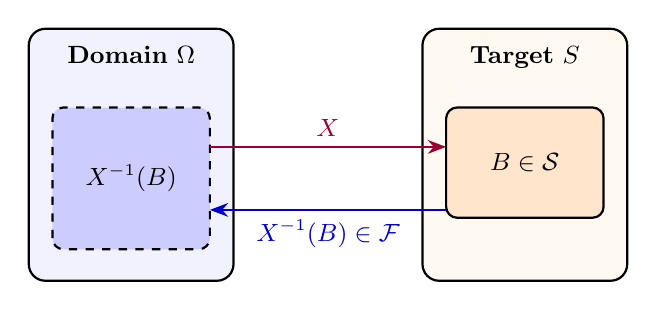
\begin{tikzpicture}[font=\small, >=Stealth]
  % Domain
  \draw[thick, rounded corners=6pt, fill=blue!5] (0,0) rectangle (2.6, 3.2);
  \node[anchor=north] at (1.3, 3.1) {\textbf{Domain} $\Omega$};
  \draw[thick, dashed, fill=blue!20, rounded corners=4pt] (0.3, 0.4) rectangle (2.3, 2.2);
  \node at (1.3, 1.3) {$X^{-1}(B)$};

  % Target
  \draw[thick, rounded corners=6pt, fill=orange!5] (5.0,0) rectangle (7.6, 3.2);
  \node[anchor=north] at (6.3, 3.1) {\textbf{Target} $S$};
  \draw[thick, fill=orange!20, rounded corners=4pt] (5.3, 0.8) rectangle (7.3, 2.2);
  \node at (6.3, 1.5) {$B \in \mathcal{S}$};

  % Arrows
  \draw[->, thick, purple!80!black] (2.3, 1.7) -- node[above] {$X$} (5.3, 1.7);
  \draw[<-, thick, blue!80!black] (2.3, 0.9) -- node[below] {$X^{-1}(B) \in \mathcal{F}$} (5.3, 0.9);
\end{tikzpicture}
\end{document}